\documentclass[a4paper,12pt]{article}
\usepackage[utf8]{inputenc}
\usepackage[T1]{fontenc}
\usepackage{lmodern}
\usepackage{graphicx}
\usepackage{amsmath}
\usepackage{amssymb}
\usepackage{color}
\usepackage{braket}
\usepackage{vmargin}
\usepackage[colorlinks=true, linkcolor=blue]{hyperref}
\usepackage{xcolor}
\usepackage{listings}

\setmarginsrb{2.5cm}{2.cm}{2.5cm}{2.cm}{0cm}{0cm}{0cm}{1cm}
\DeclareMathOperator{\R}{Ref}
\DeclareMathOperator{\T}{Tar}
\DeclareMathOperator{\Tr}{Tr}

\definecolor{vsKeyword}{RGB}{0,0,255}
\definecolor{vsString}{RGB}{163,21,21}
\definecolor{vsComment}{RGB}{0,128,0}
\definecolor{vsBackground}{RGB}{245,245,245}

\lstset{
    backgroundcolor=\color{vsBackground},
    basicstyle=\ttfamily\small,
    keywordstyle=\color{vsKeyword}\bfseries,
    stringstyle=\color{vsString},
    commentstyle=\color{vsComment}\itshape,
    showstringspaces=false,
    tabsize=4,
    captionpos=b,
    frame=single,
    breaklines=true,
    language=Python,
}

\newcommand{\mcode}[1]{\protect\lstinline[basicstyle=\color{black}\ttfamily]!#1!}

\title{GRAPE for Transmon Qubits\\ \large \texttt{grape\_scq}}
\author{L. Van Damme}
\date{\today}

\begin{document}
\maketitle
\tableofcontents

\newpage
\section*{Overview}
\phantomsection
\addcontentsline{toc}{section}{Overview}
This Python package provides tools to optimize control pulses for transmon
qubits with GRAPE (GRadient Ascent Pulse Engineering). The qubit dynamics
are described by the Hamiltonian in the rotating-wave approximation (with
$\hbar=1$):
\begin{equation}
    H/(2\pi) = \frac{\nu_{\R}}{2}\big( u(t)\,a^{\dagger} + u^{*}(t)\,a \big)
      + (\nu_q - \nu_d)\,a^{\dagger}a
      + \frac{\alpha}{2}\,a^{\dagger 2}a^{2},
\end{equation}
where:
\begin{itemize}
    \item $\nu_{\R}$ is a reference frequency (Hz) that sets the overall drive scale.
    \item $u(t) = u_x(t) + i\,u_y(t)$ is the normalized control pulse in complex form, with $u_x(t)$ (in-phase) and $u_y(t)$ (quadrature) real and dimensionless.
    \item $\nu_q$ is the qubit frequency (the $\ket{0}\!\leftrightarrow\!\ket{1}$ transition) in Hz.
    \item $\nu_d$ is the carrier (drive) frequency in Hz.
    \item $\alpha$ is the transmon anharmonicity in Hz.
    \item $a$ and $a^{\dagger}$ are the annihilation and creation operators, truncated to the number of levels considered.
\end{itemize}

Any of $\nu_q$, $\alpha$, or the drive amplitude scale factor may be a scalar,
an array over an \emph{ensemble} of parameter values (robust optimization
against uncertain parameters), or an array over both an ensemble and time
(e.g. a drifting or oscillating detuning). Control pulses can either be
optimized directly at every timestep or restricted to a linear combination
of analytical basis functions, to produce experimentally feasible shapes and
to reduce the number of free parameters. Pulses can be constrained to
respect hardware amplitude limits. The optimizer can target either a unitary
gate on a computational subspace or a state-to-state transfer in the full
Hilbert space.

\paragraph*{Limitations.} The code supports only single or uncoupled
transmons, does not implement multi-qubit gates, does not allow for multiple
control channels with different drive frequencies, neglects relaxation
processes, and is valid only within the rotating-wave approximation.

\paragraph*{Engine.} The cost function and its exact gradient (via the
adjoint-state method, one eigendecomposition per timestep) are compiled with
Numba, so the optimizer scales well with the number of timesteps, ensemble
members, and analytic-basis coefficients.

\section*{Requirements}
\phantomsection
\addcontentsline{toc}{section}{Requirements}
This package requires numpy, numba, scipy (in particular
\mcode{scipy.optimize}), and matplotlib.

\section*{Object model}
\phantomsection
\addcontentsline{toc}{section}{Object model}
A problem is assembled from a small number of explicit, composable objects:
\begin{itemize}
    \item \mcode{Transmon} --- the physical system: \mcode{n_levels}, \mcode{frequency}, \mcode{anharmonicity}, \mcode{amplitude_scale}, \mcode{carrier_frequency}.
    \item \mcode{GateTarget(matrix, subspace)} / \mcode{StateTarget(initial, target)} --- the optimization target.
    \item \mcode{OptimizationProblem(system, target, n_steps, dt, ...)} --- composes the system, the target, the time grid and, optionally, an analytic pulse basis (\mcode{ux_basis}/\mcode{uy_basis}).
    \item \mcode{GrapeOptimizer(max_iter=..., ...)} --- \mcode{optimizer.optimize(problem, initial_pulse)} returns a \mcode{Result}.
    \item \mcode{initial_guess} --- generators (\mcode{cos_drag}, \mcode{random_fourier}, \mcode{random_symmetric_antisymmetric}, \mcode{constant}, \mcode{zero}) producing an initial \mcode{Pulse}.
    \item \mcode{Result} --- the optimized pulse and convenience methods: \mcode{.plot_pulse()}, \mcode{.population(...)}, \mcode{.fidelity_map()}, \mcode{.summary()}.
\end{itemize}

\newpage
\section*{Example 1: Leakage-Free NOT Gate\\ \mcode{examples/01\_leakage\_free\_gate.ipynb}}
\phantomsection
\addcontentsline{toc}{section}{Example 1: Leakage-Free NOT Gate}

\paragraph*{General problem.}
We consider a three-level system driven on resonance.
The system Hamiltonian under the rotating-wave approximation is given by
\[
    H(t) = \frac{2\pi \nu_{\R}}{2}\big( u(t) \, a^{\dagger} + u^{*}(t) \, a \big)
         + \frac{2\pi \alpha}{2} \, a^{\dagger 2} a^{2},
\]
where $\alpha=-100$~MHz and $\nu_{\R}$ is set to $10$~MHz.
To account for three energy levels, the operators $a$ and $a^{\dagger}$ are truncated as
\[
    a = \ket{0}\bra{1} + \sqrt{2}\ket{1}\bra{2},
    \;\;
    a^{\dagger} = \ket{1}\bra{0} + \sqrt{2}\ket{2}\bra{1}.
\]
The goal is to optimize the pulse shape $u(t)$ to implement the gate
\[
    U_{\mathrm{T}} = \begin{pmatrix}
        0 & 1 \\
        1 & 0
    \end{pmatrix}
\]
on the computational subspace defined by $\ket{0}$ and $\ket{1}$.
The time is discretized into $120$ steps of $0.1$~ns, corresponding to a $12$~ns-long control pulse.

From a control perspective, this problem is underconstrained, meaning that
infinitely many pulse shapes can reach the target to numerical precision. To
select among these degenerate solutions, we minimize the pulse energy
\[(2\pi\nu_R)^2\int_0^T  u_x^2(t)+u_y^2(t)\,dt,\]
which restricts the search to solutions that achieve the target while using
minimal control amplitude.

\paragraph*{Problem setup.}
\begin{lstlisting}
system = Transmon(
    n_levels=3,            # Number of energy levels
    anharmonicity=-100e6,  # Anharmonicity in Hz
)
target = GateTarget(
    matrix=[[0, 1], [1, 0]],  # Target gate (NOT gate)
    subspace=[0, 1],          # Computational states indices
)
problem = OptimizationProblem(
    system, target,
    n_steps=120,               # Number of time steps
    dt=0.1e-9,                 # Timestep in s.
    reference_amplitude=10e6,  # Reference pulse amplitude
)
\end{lstlisting}
Note that the carrier and qubit frequencies do not need to be specified for
this simple problem, as the drive is assumed to be on-resonance with the
qubit transition by default.

\paragraph*{Initial pulse guess.} We use a DRAG-like pulse of the form
\[
    u_{x,i}(t) = A \sin\!\left(\tfrac{\pi t}{T}\right),
    \quad
    u_{y,i}(t) = B \cos\!\left(\tfrac{\pi t}{T}\right),
\]
where the parameters $A$ and $B$ are internally fit to minimize leakage under
the problem's own system and duration, generated with:
\begin{lstlisting}
pulse0 = initial_guess.cos_drag(problem, theta=np.pi)
\end{lstlisting}
Here, \mcode{theta=np.pi} specifies that the DRAG guess should implement a
$\pi$-rotation in the computational basis.

\paragraph*{Optimization.} We search for a minimum-energy solution:
\begin{lstlisting}
optimizer = GrapeOptimizer(
    max_iter=500,          # Maximum number of iterations
    minimize_energy=True,  # Find minimum-energy solution
)
result = optimizer.optimize(problem, pulse0)
\end{lstlisting}
which returns a \mcode{Result} holding the optimal pulse and its fidelity.

\paragraph*{Results.} The pulse components in Hz are obtained and plotted with:
\begin{lstlisting}
result.plot_pulse(compare_to_initial=True)
\end{lstlisting}
The resulting pulse is shown in Fig.~\ref{FigEx01}, together with the
leakage population $|\!\braket{2|\psi(t)}\!|^2$ obtained from
\mcode{result.population(0, 2)} and \mcode{result.population(1, 2)}. The
optimized pulse reaches a gate fidelity of $100.000\,\%$ (to the precision
shown), essentially suppressing leakage to $\ket{2}$, starting from a
$98.005\,\%$-fidelity DRAG guess. The complete script is provided in
\mcode{examples/01\_leakage\_free\_gate.ipynb}.
\begin{figure}[h]
\centering
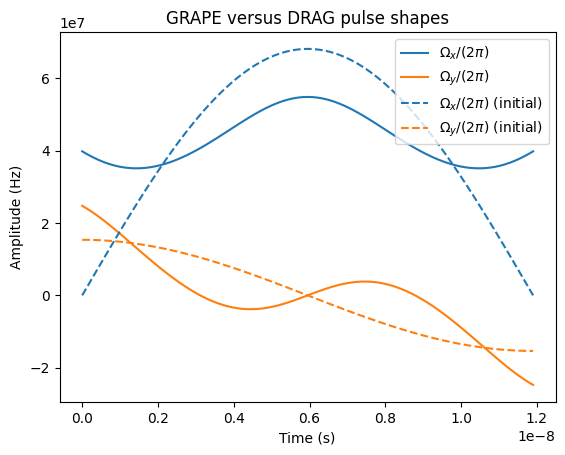
\includegraphics[width=0.48\textwidth]{figures/01_leakage_free_gate_1.png}
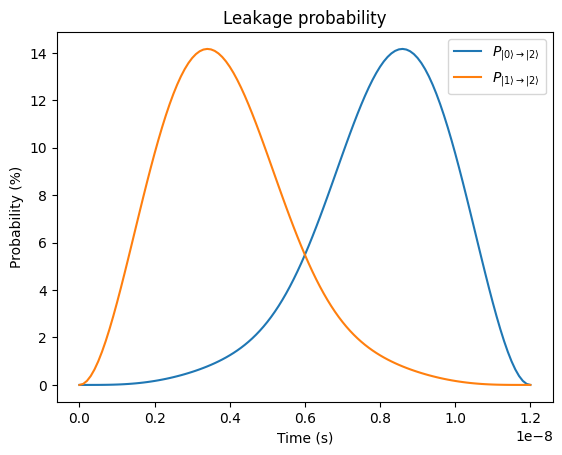
\includegraphics[width=0.48\textwidth]{figures/01_leakage_free_gate_2.png}
\caption{Left panel: Pulse shapes in Hz before (dashed) and after (solid) optimization. Right panel: Leakage to state $\ket{2}$ as a function of time.\label{FigEx01}}
\end{figure}

\section*{Example 2: Two-Photon Transition\\
\mcode{examples/02\_two\_photon\_transition.ipynb}}
\phantomsection
\addcontentsline{toc}{section}{Example 2: Two-Photon Transition}

\paragraph*{General problem.}
We consider a transmon with anharmonicity $\alpha=-200~\mathrm{MHz}$ and
$\ket{0}\!\leftrightarrow\!\ket{1}$ frequency $\nu_q=5~\mathrm{GHz}$, driven
at the two-photon resonance
\[
\nu_d=\nu_q+\alpha/2=\nu_{02}/2.
\]
In the frame rotating at $\nu_d$ and under the RWA, the control Hamiltonian is
\[
    H = \frac{2\pi \nu_{\R}}{2}\big( u(t) \, a^{\dagger} + u^{*}(t) \, a \big)
      - \frac{2\pi\alpha}{4} \, a^{\dagger} a
      + \frac{2\pi \alpha}{2} \, a^{\dagger 2} a^{2}.
\]
To capture leakage, we simulate the system with four energy levels, with $a$
and $a^\dagger$ truncated accordingly. Starting from $\ket{\psi(0)}=\ket{0}$,
the objective is to optimize $u(t)$ to transfer the state to $\ket{2}$, such
that $|\!\braket{2|\psi(T)}\!|^2=1$. The time is discretized into $200$ steps
of $0.1$~ns, corresponding to $T=20$~ns. As in Example~1, this problem is
underconstrained, and we again minimize the pulse energy to select a
minimum-amplitude solution.

\paragraph*{Problem setup.}
\begin{lstlisting}
system = Transmon(
    n_levels=4,
    anharmonicity=-200e6,
    frequency=5e9,
    carrier_frequency=5e9 - 200e6/2,  # Two-photon resonance
)
target = StateTarget(initial=[1, 0, 0, 0], target=[0, 0, 1, 0])
problem = OptimizationProblem(system, target, n_steps=200, dt=0.1e-9,
                               reference_amplitude=100e6)
\end{lstlisting}
Note that the computational subspace does not need to be specified for a
\mcode{StateTarget}: the initial and target states are defined in the full
Hilbert space.

\paragraph*{Initial pulse guess.} We use a symmetric/antisymmetric random
low-order Fourier series:
\begin{lstlisting}
pulse0 = initial_guess.random_symmetric_antisymmetric(problem)
\end{lstlisting}

\paragraph*{Optimization.} We again search for a minimum-energy solution:
\begin{lstlisting}
optimizer = GrapeOptimizer(max_iter=1000, minimize_energy=True)
result = optimizer.optimize(problem, pulse0)
\end{lstlisting}

\paragraph*{Results.} The pulse is visualized with
\mcode{result.plot_pulse(compare_to_initial=False)}. The resulting pulse is
shown in Fig.~\ref{FigEx02}, together with the transition probabilities
$P_{0\to1}$, $P_{0\to2}$ (target) and $P_{0\to3}$ (leakage), obtained from
\mcode{result.population(0, k)}. The complete script is provided in
\mcode{examples/02\_two\_photon\_transition.ipynb}.
\begin{figure}[h]
\centering
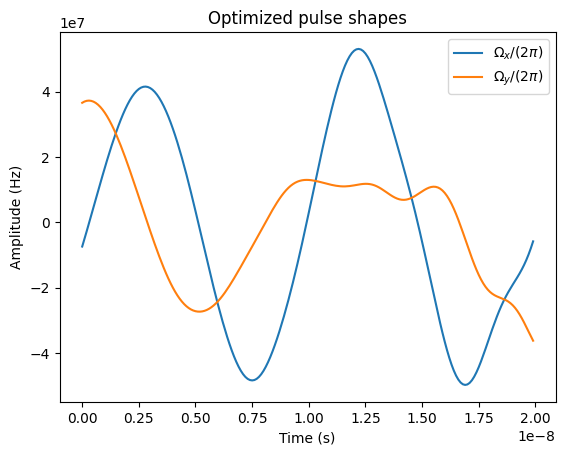
\includegraphics[width=0.48\textwidth]{figures/02_two_photon_transition_1.png}
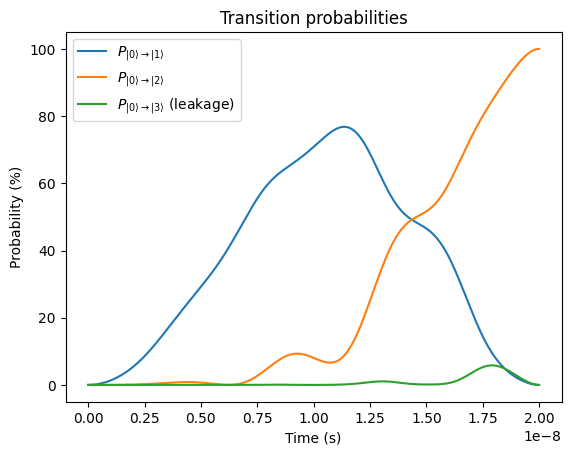
\includegraphics[width=0.48\textwidth]{figures/02_two_photon_transition_2.png}
\caption{Left: Pulse amplitudes (in Hz) implementing a two-photon transition from $\ket{0}$ to $\ket{2}$. Right: Transition probabilities as a function of time. \label{FigEx02}}
\end{figure}

\newpage
\section*{Example 3: Analytically Shaped Hadamard Gate\\
\mcode{examples/03\_analytic\_pulse\_shaping.ipynb}}
\phantomsection
\addcontentsline{toc}{section}{Example 3: Analytically Shaped Hadamard Gate}

\paragraph*{General problem.}
We consider the same three-level, on-resonance system as in Example~1, now
with $\alpha=-200$~MHz, and target a Hadamard gate,
\[
    U_{\mathrm{T}} = \tfrac{1}{\sqrt{2}}\begin{pmatrix}
        1 & 1 \\
        1 & -1
    \end{pmatrix},
\]
on the computational subspace spanned by $\ket{0}$ and $\ket{1}$. In
contrast to Examples~1 and~2, the pulse shape is restricted to a basis of
analytical functions:
\[
\begin{aligned}
u_x(t) &= \sum_{k=1}^{3} a_{x_k} \sin\!\left(\tfrac{(2k-1)\pi t}{T}\right), \\
u_y(t) &= \sum_{k=1}^{3} a_{y_k} \cos\!\left(\tfrac{(2k-1)\pi t}{T}\right),
\end{aligned}
\]
and the optimizer searches for the coefficients $\{a_{x_k}, a_{y_k}\}$ that
realize the target gate. The control pulse is discretized into $160$ time
steps of $0.1$~ns, i.e. a total duration of $16$~ns.

\paragraph*{Problem setup.} Instead of optimizing the pulse directly at each
time step, the control fields are described as a combination of analytical
functions, passed to \mcode{OptimizationProblem} as \mcode{ux_basis} and
\mcode{uy_basis}:
\begin{lstlisting}
n_steps, n_coeffs = 160, 3
tau = np.linspace(0, 1, n_steps)
fx = np.array([np.sin((2*n+1)*np.pi*tau) for n in range(n_coeffs)])
fy = np.array([np.cos((2*n+1)*np.pi*tau) for n in range(n_coeffs)])

system = Transmon(n_levels=3, anharmonicity=-200e6)
target = GateTarget(matrix=np.array([[1, 1], [1, -1]])/np.sqrt(2), subspace=[0, 1])
problem = OptimizationProblem(system, target, n_steps=n_steps, dt=0.1e-9,
                               ux_basis=fx, uy_basis=fy)
\end{lstlisting}
With this setup, the optimizer no longer works on $u_x$ and $u_y$ at each
time step, but only on the coefficients $a_{x_k}$ and $a_{y_k}$.

\paragraph*{Initial pulse guess.} We use a random low-order Fourier guess
for the coefficients:
\begin{lstlisting}
pulse0 = initial_guess.random_fourier(problem, n_coeffs=n_coeffs)
\end{lstlisting}

\paragraph*{Optimization.}
\begin{lstlisting}
result = GrapeOptimizer(max_iter=500).optimize(problem, pulse0)
\end{lstlisting}

\paragraph*{Results.} The pulse component $u_x(t)$ and $u_y(t)$ are
recovered from the coefficients via the basis stored on \mcode{problem} and
visualized with \mcode{result.plot_pulse()}. The resulting pulse is shown
in Fig.~\ref{FigEx03}, together with the transition probabilities
(including leakage to $\ket{2}$). The complete script is provided in
\mcode{examples/03\_analytic\_pulse\_shaping.ipynb}.
\begin{figure}[h]
\centering
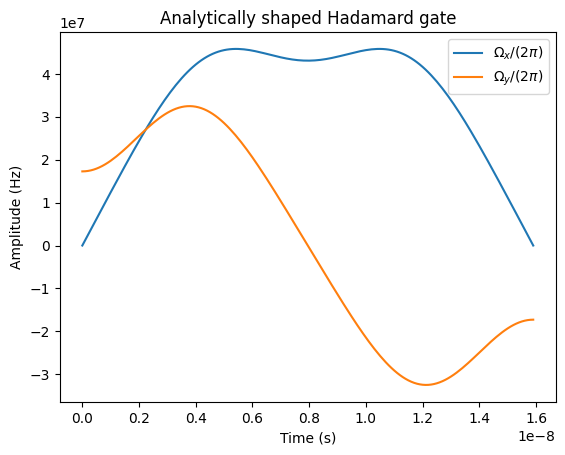
\includegraphics[width=0.48\textwidth]{figures/03_analytic_pulse_shaping_1.png}
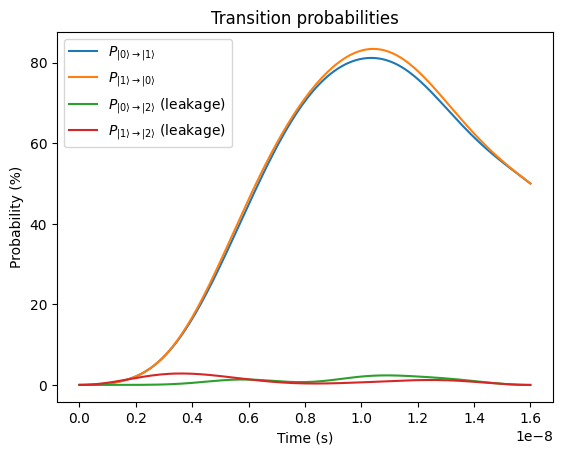
\includegraphics[width=0.48\textwidth]{figures/03_analytic_pulse_shaping_2.png}
\caption{Left: Analytically shaped pulse implementing a Hadamard gate. Right: Transition probabilities, including leakage to $\ket{2}$.\label{FigEx03}}
\end{figure}

\newpage
\section*{Example 4: Robust Fourier Pulse\\
\mcode{examples/04\_robust\_fourier\_pulse.ipynb}}
\phantomsection
\addcontentsline{toc}{section}{Example 4: Robust Fourier Pulse}

\paragraph*{General problem.}
We consider a transmon system subject to both pulse amplitude deviations
and detuning errors. Within the rotating-wave approximation, the system
Hamiltonian is
\[
    H(\epsilon,\delta,t) = \frac{2\pi \nu_{\R}}{2}\,(1+\epsilon)\big( u(t)\,a^{\dagger} + u^{*}(t)\,a \big)
    + 2\pi(\nu_q - \nu_d + \delta)\,a^{\dagger}a
    + \frac{2\pi \alpha}{2}\,a^{\dagger 2} a^{2},
\]
where $\alpha = -200$~MHz, $\nu_{\R} = 5$~MHz, and $\nu_q = \nu_d = 5$~GHz.
Here $\epsilon$ (dimensionless) models a relative drive-amplitude error,
while $\delta$ (in Hz) is a detuning error. The goal is to design a control
pulse $u(t)$ implementing an $X_{\pi/2}$ gate,
\[
    U_{\mathrm{T}} = \tfrac{1}{\sqrt{2}}\begin{pmatrix}
        1 & -i \\
        -i & 1
    \end{pmatrix},
\]
on the computational subspace $\{\ket{0},\ket{1}\}$, that remains accurate
for all $(\epsilon,\delta)$ within
$\epsilon \in [-0.1,\,0.1]$, $\delta \in [-0.2,\,0.2]~\mathrm{MHz}$. In
practice, $\epsilon$ and $\delta$ are discretized on a $5\times5$ grid, and
the optimizer minimizes the average infidelity over the grid,
\[
    J = \frac{1}{N_{\epsilon}N_{\delta}}\sum_{n=1}^{N_{\epsilon}} \sum_{m=1}^{N_{\delta}} \left( 1 - \tfrac{1}{2} \Big|\Tr\big(U_T^{\dagger} U_{nm}^{01}(T)\big)\Big|^2 \right).
\]
As in Example~3, the pulse is restricted to a Fourier basis,
\[
u_x(t) = \sum_{k=1}^{5} a_k \sin\!\left(\tfrac{(2k-1)\pi t}{T}\right), \quad
u_y(t) = \sum_{k=1}^{5} b_k \sin\!\left(\tfrac{2k\pi t}{T}\right),
\]
with an amplitude constraint $\nu_{\R}u_x(t),\,\nu_{\R}u_y(t)\leq 15~\mathrm{MHz}$.
The control pulse is discretized into $200$ steps of $0.5$~ns ($100$~ns total).

\paragraph*{Problem setup.} The robustness grid is built with
\mcode{Transmon.sweep}, which meshes the swept keyword arguments and
remembers the grid shape for later fidelity-map plotting:
\begin{lstlisting}
Na, Nd = 5, 5
amp_error = np.linspace(-0.1, 0.1, Na)     # Amplitude error [-10%, 10%]
detuning = 0.2e6 * np.linspace(-1, 1, Nd)  # Detuning [-0.2 MHz, 0.2 MHz]

system = Transmon.sweep(
    frequency=5e9 + detuning,
    amplitude_scale=1 + amp_error,
    anharmonicity=-200e6,
)
target = GateTarget(matrix=np.array([[1, -1j], [-1j, 1]])/np.sqrt(2), subspace=[0, 1])

n_steps, n_coeffs = 200, 5
fx = symmetric_fourier_basis(n_steps, n_coeffs)
fy = antisymmetric_fourier_basis(n_steps, n_coeffs)
problem = OptimizationProblem(system, target, n_steps=n_steps, dt=0.5e-9,
                               reference_amplitude=5e6, ux_basis=fx, uy_basis=fy)
\end{lstlisting}

\paragraph*{Initial pulse guess.}
\begin{lstlisting}
pulse0 = initial_guess.cos_drag(problem, theta=np.pi/2)
\end{lstlisting}

\paragraph*{Optimization.} We impose the amplitude constraint via
\mcode{max_in_phase}/\mcode{max_quadrature}:
\begin{lstlisting}
optimizer = GrapeOptimizer(max_iter=2000, max_in_phase=15e6, max_quadrature=15e6)
result = optimizer.optimize(problem, pulse0)
\end{lstlisting}

\paragraph*{Results.} The pulse is shown in the left panel of
Fig.~\ref{FigEx04}. To visualize robustness, the same optimized pulse is
re-evaluated on a finer $(\delta,\epsilon)$ grid via
\mcode{problem.with_system(fine_system)} and
\mcode{analysis.fidelity_map(...)}, producing the fidelity map on the right.
The complete script is provided in
\mcode{examples/04\_robust\_fourier\_pulse.ipynb}.
\begin{figure}[h]
\centering
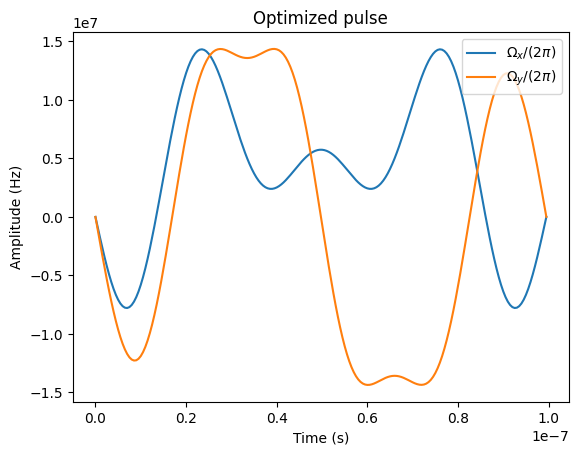
\includegraphics[width=0.48\textwidth]{figures/04_robust_fourier_pulse_1.png}
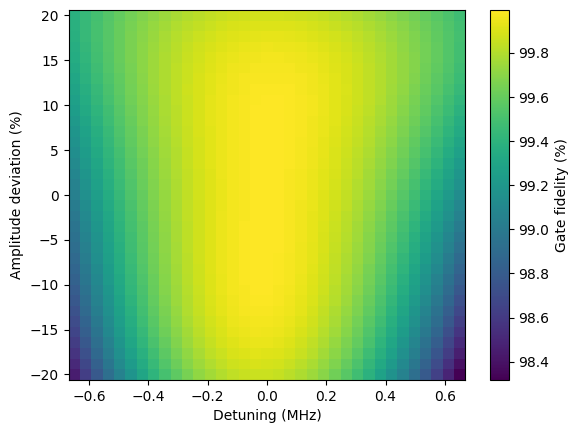
\includegraphics[width=0.48\textwidth]{figures/04_robust_fourier_pulse_2.png}
\caption{Left: Pulse amplitudes (in Hz) implementing a robust $X_{\pi/2}$ gate. Right: Gate fidelity as a function of detuning and amplitude deviation, evaluated on a finer grid than the one used for optimization.\label{FigEx04}}
\end{figure}

\newpage
\section*{Example 5: Selective Pulse\\
\mcode{examples/05\_selective\_pulse.ipynb}}
\phantomsection
\addcontentsline{toc}{section}{Example 5: Selective Pulse}

\paragraph*{General problem.}
We consider a two-level quantum system with dynamics governed by
\[
    H(\delta,t) = \frac{2\pi \nu_{\R}}{2}\big( u(t)\,a^{\dagger} + u^{*}(t)\,a \big)
    + 2\pi(\nu_q - \nu_d + \delta)\,a^{\dagger}a,
\]
where $\nu_q = \nu_d = 5$~GHz and the detuning $\delta$ takes one of two
values, $\pm 2.5$~MHz. Since only the two lowest levels are considered, the
ladder operators are truncated as $a=\ket{0}\bra{1}$,
$a^{\dagger}=\ket{1}\bra{0}$. The goal is to design a control pulse $u(t)$
that maps $\ket{0}$ to a \emph{different} outcome depending on the
detuning:
\[\begin{cases}
   \ket{0}\to\ket{0} & \text{if } \delta = -2.5~\mathrm{MHz}, \\
   \ket{0}\to\ket{1} & \text{if } \delta = +2.5~\mathrm{MHz},
\end{cases}
\]
subject to the amplitude constraint $|u(t)|\nu_{\R}\leq 8~\mathrm{MHz}$. The
control pulse is discretized into $120$ time steps of $1$~ns ($120$~ns
total). Selectivity is achieved by simultaneously optimizing over the two
detuning values as two \emph{ensemble members} of the same \mcode{Transmon},
each carrying its own target state.

\paragraph*{Problem setup.} Both ensemble members start in $\ket{0}$;
member~0 (detuning $-2.5$~MHz) targets $\ket{0}$, member~1 ($+2.5$~MHz)
targets $\ket{1}$:
\begin{lstlisting}
system = Transmon(
    n_levels=2,
    frequency=5e9 + np.array([-2.5e6, 2.5e6]),
    carrier_frequency=5e9,
)
target = StateTarget(initial=[[1, 0], [1, 0]], target=[[1, 0], [0, 1]])
problem = OptimizationProblem(system, target, n_steps=120, dt=1e-9)
\end{lstlisting}

\paragraph*{Initial pulse guess.} We start from a constant drive along $x$:
\begin{lstlisting}
pulse0 = initial_guess.zero(problem)
pulse0.ux[:] = 1.0
\end{lstlisting}

\paragraph*{Optimization.}
\begin{lstlisting}
optimizer = GrapeOptimizer(max_iter=2000, max_amplitude=8e6)
result = optimizer.optimize(problem, pulse0)
\end{lstlisting}

\paragraph*{Results.} The resulting pulse resembles a Ramsey experiment,
with the pulse switched off during an intermediate free-evolution window
(Fig.~\ref{FigEx05}, left), during which the two detunings accumulate
opposite phases that are resolved by the final pulse segment into the two
different target outcomes (right panel). This solution is analogous to the
time-optimal solution reported for the equivalent (swapped-target) problem
in Phys.\ Rev.\ A~98, 043421. The complete script is provided in
\mcode{examples/05\_selective\_pulse.ipynb}.
\begin{figure}[h]
\centering
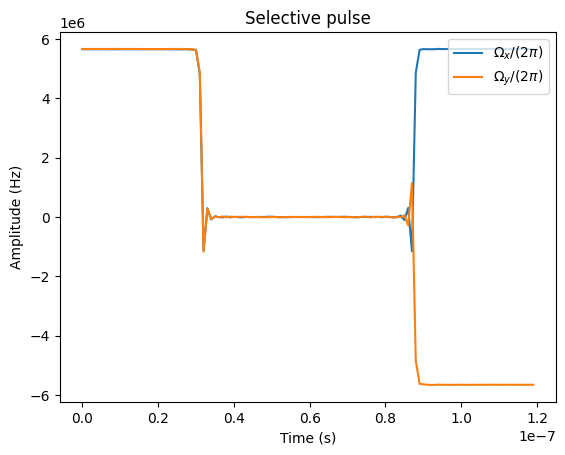
\includegraphics[width=0.48\textwidth]{figures/05_selective_pulse_1.png}
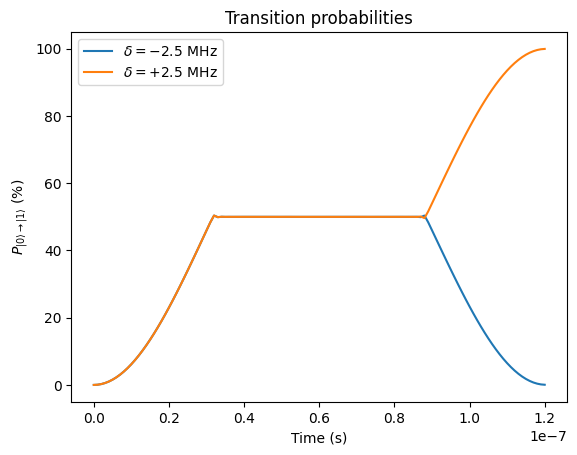
\includegraphics[width=0.48\textwidth]{figures/05_selective_pulse_2.png}
\caption{Left panel: Optimal pulse shape in Hz. Right panel: Transition probability $P_{0\to1}$ as a function of time, for both detunings.\label{FigEx05}}
\end{figure}

\newpage
\section*{Example 6: Time-Dependent Detuning Robustness\\
\mcode{examples/06\_time\_dependent\_detuning.ipynb}}
\phantomsection
\addcontentsline{toc}{section}{Example 6: Time-Dependent Detuning Robustness}

\paragraph*{General problem.}
We revisit the leakage-free NOT gate of Example~1 ($\alpha=-100$~MHz, three
levels), but now require robustness against a time-dependent detuning of
the form
\[
    \delta(t) = A\cos(2\pi\omega t),
\]
over a grid of $\omega \in [0,\,10]$~MHz and $A \in [-5,\,5]$~MHz. Because
\mcode{Transmon.frequency} accepts a 2-D array of shape
\mcode{(n\_ensemble, n\_steps)}, each grid point $(\omega_n, A_m)$ becomes
one ensemble member with its own detuning \emph{trace} $\delta_{nm}(t)$,
rather than a single constant offset as in Example~4. As in Example~4, the
optimizer minimizes the ensemble-averaged infidelity over the grid. The
pulse is restricted to a symmetric/antisymmetric Fourier basis with $10$
harmonics per quadrature and constrained to
$(u_x^2(t)+u_y^2(t))^{1/2}\nu_{\R}\leq 20$~MHz. The control pulse is
discretized into $150$ steps of $1$~ns ($150$~ns total).

\paragraph*{Problem setup.}
\begin{lstlisting}
n_steps, dt = 150, 1e-9
tc = np.arange(n_steps) * dt
Nw, NA = 5, 5
w = np.linspace(0, 10e6, Nw)
A = np.linspace(-5e6, 5e6, NA)
wGrid, AGrid = np.meshgrid(w, A)
detuning = AGrid.ravel()[:, None] * np.cos(2*np.pi*wGrid.ravel()[:, None] * tc[None, :])

system = Transmon(n_levels=3, frequency=5e9 + detuning,
                   carrier_frequency=5e9, anharmonicity=-100e6)
system.grid_shape = wGrid.shape          # Remember the grid for later plotting
system.grid_axes = {"w": w, "A": A}

target = GateTarget(matrix=[[0, 1], [1, 0]], subspace=[0, 1])

n_coeffs = 10
fx = symmetric_fourier_basis(n_steps, n_coeffs)
fy = antisymmetric_fourier_basis(n_steps, n_coeffs)
problem = OptimizationProblem(system, target, n_steps=n_steps, dt=dt,
                               ux_basis=fx, uy_basis=fy)
\end{lstlisting}

\paragraph*{Initial pulse guess.}
\begin{lstlisting}
pulse0 = initial_guess.cos_drag(problem, theta=np.pi)
\end{lstlisting}

\paragraph*{Optimization.}
\begin{lstlisting}
optimizer = GrapeOptimizer(max_iter=2000, max_amplitude=20e6)
result = optimizer.optimize(problem, pulse0)
\end{lstlisting}

\paragraph*{Results.} The optimized pulse is shown in
Fig.~\ref{FigEx06pulse}. As in Example~4, the optimized pulse and the
initial DRAG guess are then both re-evaluated on a finer $55\times55$
$(\omega, A)$ grid, via \mcode{problem.with_system(fine_system)} and
\mcode{analysis.fidelity_map(...)}, to produce the fidelity maps in
Fig.~\ref{FigEx06map}: the optimized pulse maintains high fidelity over a
much wider region of the $(\omega,A)$ plane than the DRAG guess. The
complete script is provided in
\mcode{examples/06\_time\_dependent\_detuning.ipynb}.
\begin{figure}[h]
\centering
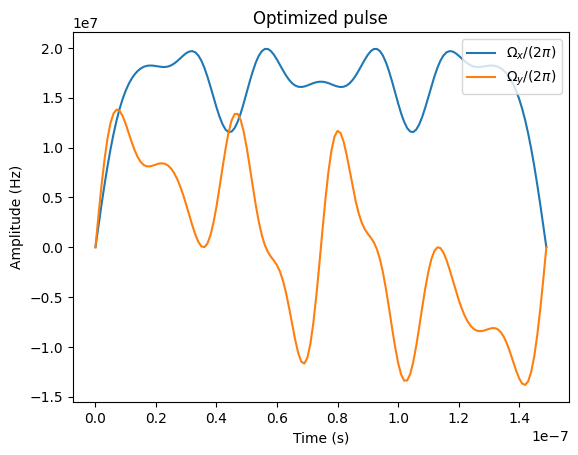
\includegraphics[width=0.6\textwidth]{figures/06_time_dependent_detuning_1.png}
\caption{Optimized pulse, robust to a time-dependent detuning $\delta(t)=A\cos(2\pi\omega t)$.\label{FigEx06pulse}}
\end{figure}
\begin{figure}[h]
\centering
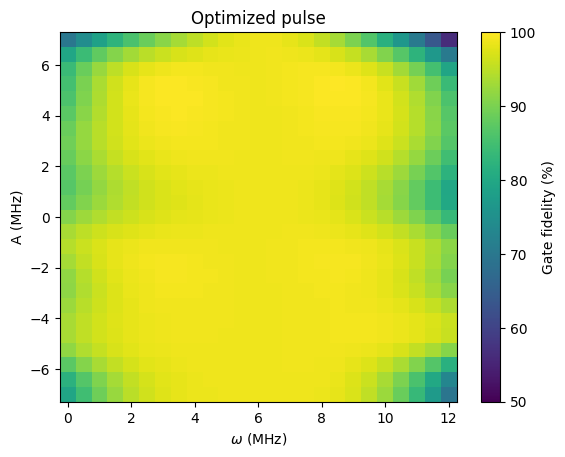
\includegraphics[width=0.48\textwidth]{figures/06_time_dependent_detuning_2.png}
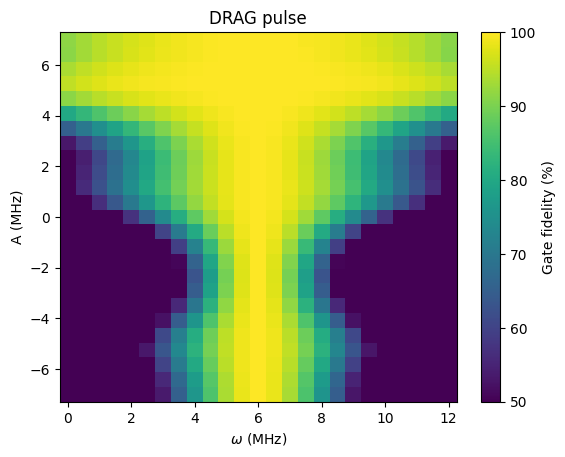
\includegraphics[width=0.48\textwidth]{figures/06_time_dependent_detuning_3.png}
\caption{Gate fidelity as a function of $(\omega, A)$, evaluated on a finer grid than the one used for optimization. Left: optimized pulse. Right: initial DRAG guess.\label{FigEx06map}}
\end{figure}

\end{document}
